\section{Extending Reo for Stochastic and Timed Behavior}
\label{sec:reo}

\subsection{Reo}

Reo is a channel-based exogenous coordination language proposed by F. Arbab in \cite{ARBAB2004}, where concurrency protocols are manifested as \emph{connectors}. Basically, connectors are constructed through a compositional approach: complex ones are composed of simpler ones, where the atomic ones are called \emph{channels}. Channels are glued on \emph{nodes}, and they together perform the behavior of connectors.

\vspace{.5em}

\noindent\emph{Nodes.} There are three types of nodes in Reo: \emph{source nodes}, \emph{sink nodes} and \emph{mixed nodes}, as shown in Fig.~\ref{fig:typeofnodes}.

\begin{figure}[H]
    \centering
    \begin{tikzpicture}[->,>=stealth',shorten >=1pt,auto,node distance=1.6cm,
  semithick]
    \tikzstyle{every node}=[font=\small]

    % source node
    \ionode{(P-1)}{(-4.5,0)}{}
    \sync{(P-1)}{(-3.5,0.5)}{}
    \sync{(P-1)}{(-3.5,-0.5)}{}

    \node (nt1) at (-4,-1) {Source Node};
    % sink node
    \ionode{(S-1)}{(-1,0)}{}
    \sync{(-2,0.5)}{(S-1)}{}
    \sync{(-2,-0.5)}{(S-1)}{}

    \node (nt2) at (-1.5,-1) {Sink Node};

    % mixed node
    \mixednode{(M-4)}{(1,0)}{}
    \sync{(0,0.5)}{(M-4)}{}
    \sync{(0,0)}{(M-4)}{}
    \sync{(0,-0.5)}{(M-4)}{}
    \sync{(M-4)}{(2,0.5)}{}
    \sync{(M-4)}{(2,-0.5)}{}

    \node (nt3) at (1,-1) {Mixed Node};

\end{tikzpicture}
    \caption{Three Types of Nodes}
    \label{fig:typeofnodes}
\end{figure}

Essentially, a \emph{source node} performs \emph{replicating} behavior. That is, any coming data values will be broadcasted synchronously if and only if all its successors are ready to accept. A \emph{sink node} performs \emph{merging} behavior, accepting data values from its predecessors \ly{randomly} (this can be a non-deterministic choice if all predecessors are ready to write). And a \emph{mixed node}, literally, performs both behavior at the same time, randomly picking one input and broadcasting it to all outputs.

\vspace{.5em}
\noindent\emph{Channels.} As the basic functional units in Reo, channels are supposed to describe basic coordination behavior among \emph{channel ends}. A channel ends can be either a \emph{source end} or a \emph{sink end}, indicating the direction of its data flow. A set of primitive channels can be found in Fig.~\ref{fig:basicchannels}, where we use arrows to indicate the type of channel ends.

\begin{figure}[H]
    \centering
    \begin{tikzpicture}[scale=1.4]

\tikzstyle{every node}=[font=\small]
\tikzstyle{label}=[draw=none]

\draw (0.5, -0.3) node[label] {Sync};
\draw (1.7, -0.3) node[label] {LossySync};
\draw (2.9, -0.3) node[label] {SyncDrain};
\draw (4.1, -0.3) node[label] {AsyncDrain};
\draw (5.3, -0.3) node[label] {Fifo1};
\draw (6.5, -0.3) node[label] {Filter$\langle P\rangle$};

\sync{(0,0)}{(1,0)}{}
\lossysync{(1.2,0)}{(2.2,0)}{}
\syncdrain{(2.4,0)}{(3.4,0)}{}
\asyncdrain{(3.6,0)}{(4.6,0)}{}
\fifoe{(4.8,0)}{(5.8,0)}{}
\filter{(6.0, 0)}{(7.0, 0)}{node[above] {P}}

\end{tikzpicture}
    \caption{Primitive Channels}
    \label{fig:basicchannels}
\end{figure}

Channels can be either \emph{synchronous} or \emph{asynchronous}. A channel is \emph{synchronous} if and only if the read and write operations on its channel ends are always performed simultaneously. The behavior of the primitive channels shown in Fig.\ref{fig:basicchannels} are specified as follows.

\begin{description}
    \item \emph{Sync(A:source,B:sink)} is a \emph{synchronous} channel that delivers data values from its source end $A$ to its sink end $B$. A synchronous channel is fired only when $A$ is prepared for reading and $B$ is ready for writing. 
    \item \emph{LossySync(A:source,B:sink)}
    is an \emph{input-enabled synchronous} channel with a source end $A$ and a sink end $B$. Such channels are always prepared to accept data from $A$. However, the transmission process could be unreliable. If $B$ is also ready for writing, the received value will be sent to $B$. Otherwise the value will be dropped immediately.
    \item \emph{SyncDrain(A\:B:source)} is a \emph{synchronous} channel with two source ends $A$ and $B$. It only accepts input from both $A$ and $B$ simultaneously and drop them together after being received.
    \item \emph{AsyncDrain(A\:B:source)} is an asynchronous variation of \emph{SyncDrain}. The most important difference is that it accepts data only from one end at a time. If both ends are ready to read, one of them (randomly picked) should wait.
    \item \emph{FIFO1(A:source,B:sink)} is an asynchronous channel with a source end $A$ and a sink end $B$. A FIFO1 channel can temporarily store one data value from its source end $A$ for arbitrary duration, and deliver it anytime when $B$ is ready to write. When the buffer is full, a FIFO1 cannot accept any more data values.
    \item \emph{Filter$\langle P\rangle$(A:source,B:sink)}
    is a synchronous channel with a source end $A$, a sink end $B$ and a boolean function $P$ as its parameter. When data comes to end A, first we have to check whether the value satisfies the filter predicate $P$. If the answer is yes, the channel will behave just as \emph{Sync}, otherwise the value will be simply dropped.
\end{description}

\noindent\emph{Composition.} Formalization of nodes sometimes becomes rather complicated, as arbitrary number of incoming and outgoing edges may be involved. Usually, we tend to introduce two ternary channels \emph{Replicator}, \emph{Merger} and use their combinations to capture the behavior of mixed nodes.

\begin{figure}[H]
    \centering
    \begin{tikzpicture}
    % replicator
    \ionode{(P-1)}{(0,0)}{}
    \ionode{(P-2)}{(1.5,0.5)}{}
    \ionode{(P-3)}{(1.5,-0.5)}{}
    \sync*{(P-1)}{(0.75,0)}{}
    \sync{(0.75,0)}{(P-2)}{}
    \sync{(0.75,0)}{(P-3)}{}

    \ionode{(M-1)}{(3,0.5)}{}
    \ionode{(M-2)}{(3,-0.5)}{}
    \ionode{(M-3)}{(4.5,0)}{}
    \sync*{(M-1)}{(3.75,0)}{}
    \sync*{(M-2)}{(3.75,0)}{}
    \sync{(3.75,0)}{(M-3)}{}
\end{tikzpicture}
    \caption{Replicator and Merger}
\end{figure}

\begin{description}
    \item \emph{Replicator(A:source,B\:C:sink)} is a \emph{synchronous} broadcast channel with a source end $A$ and two sink ends $B,C$. The channel accepts data values from $A$, and broadcasts them to $B,C$ iff. both $B$ and $C$ are ready to write.
    \item \emph{Merger(A\:B:source,C:sink)}
    is an \emph{asynchronous} channel that collects inputs from either $A$ or $B$ and sends them to $C$ simultaneously if $C$ is prepared.
\end{description}

\emph{Replicator}s and \emph{Merger}s can reduce the number of incoming and outgoing edges for mixed nodes. For example, if we replace two outgoing edges with a \emph{Replicator} channel, the number of edges would be reduced by 1. After a finite number of replacements, all the mixed nodes can be simplified as nodes with one incoming edge and one outgoing edge, which are called \emph{flow-through}.
When processing the semantics of connectors, we assume that all the mixed nodes are \emph{flow-through} ones. But in the figures we still draw the mixed nodes in their original form to make it clear and easy to understand.

\subsection{Capturing Timed and Stochastic Behavior}

In this subsection, we come up with some primitive channels, which extend Reo and make it capable to specify timed and stochastic behavior.
Compared with other formal languages, Reo provides a framework which can be easily extended by adding new channel types to the primitive channel set. Usually, new channels should be simple enough, and orthogonal to the existing ones. Following this idea, here we propose three channel types, capturing \emph{data evolution}, \emph{stochastic choice}, and \emph{time delay}.

In the following definitions, we use $\langle p \rangle$ to denote the parameter of a channel. Value of parameters should be provided while declaring the channel, and would never be updated during the execution.

\begin{figure}[t]
    \centering
    \label{fig:newchannels}
    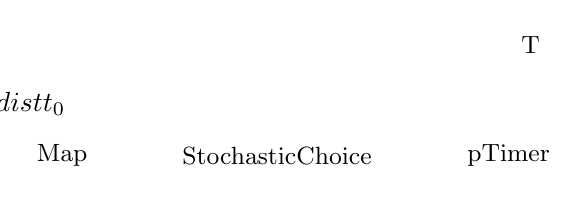
\begin{tikzpicture}[scale=1.4]

\tikzstyle{every node}=[font=\small]
\tikzstyle{label}=[draw=none]

\draw (0.75, -0.4) node[label] {Map};
\draw (2.7, -0.4) node[label] {StochasticChoice};
\draw (4.8, -0.4) node[label] {pTimer};

\draw (5, 0.6) node[label] {T};

\map{(0,0)}{(1.5,0)}{node [above=3] {$f$}}
\choice{(1.95,0)}{(3.45,0)}{node [above=0.2cm, xshift=-0.6cm] {$dist$}}
\ptimer{(4.1,0)}{(4.85, 0.6)}{(5.6,0)}{node [above=1, xshift=-0.2cm] {$t_0$}}

\end{tikzpicture}
    \caption{Extended Primitive Channels}
\end{figure}

\begin{description}
    \item \emph{Map$\langle f\rangle$(A:source,B:sink)}
        is a synchronous channel with a source end $A$, a sink end $B$ and a mapping function $f$ as its parameter. 
        A \emph{Map} channel accepts incoming values from its source end $A$ (only when $B$ is ready for writing) and then it writes $f(dA)$ to $B$ simultaneously \ly{($dA$ denotes the data accepted from $A$)}.
    
    \item \emph{StochasticChoice$\langle dist\rangle($A:source,B:sink)} is a synchronous randomizer channel that accepts data values from its source node $A$ (only when $B$ is ready for writing) and writes a random value to $B$ simultaneously. The random value is sampled from the distribution parameter $dist$.
    
    \item \emph{pTimer$\langle t_0\rangle$(A\:T:source,B:sink)} is a \emph{parameterized} version of $t$-Timer in \cite{Meng2012}. 
        The channel accepts data values from its source end $A$ and starts counting down. Then after a certain delay, it will send a TIMEOUT signal to $B$ if writable, and otherwise do nothing. In both cases, the channel will reset itself and prepare to accept the next incoming value.
        
        Value of the delay is initialized by the parameter $t_0$, and can be overridden by incoming values from the source end $T$. When the \emph{pTimer} is not in counting down stage, an incoming value from T will simply update the delay value. Otherwise the incoming value will reset it, update the delay value, and write nothing to $B$. When the new delay value is provided exactly at the same time when counting down process terminates, the channel will still generate the timeout signal.

\end{description}


